\subsection{Teil 2 - Informationsextraktion}

% https://www.diva-portal.org/smash/get/diva2:934351/FULLTEXT01.pdf
% -> Referenziert System von Hamza et al.
% -> OCR Error Correction approach von Sorio et al.


Um eine Rechnung verarbeiten zu können, müssen diverse Informationen, wie beispielsweise der Totalbetrag oder der Leistungsbezüger, aus dieser extrahiert werden. Diese Problematik der Informationsextraktion wird bereits von vielen existieren Software Lösungen zur automatisierten Verarbeitung von Rechnungen implementiert. Diese Systeme extrahieren zwei verschiedene Typen von Informationen: Informationen mit Schlüsselwörter oder Informationen aus Tabellen~\autocite{Hamza}.

Die Extraktion von Informationen aus Tabellen wurde bereits viel behandelt. Ein einfacher Ansatz von \textcite{Mandal} erreicht bereits eine Treffergenauigkeit von 97.21\%~(\cite{Mandal} in \cite{Hamza}).

\textcite{Hamza} stellen eine Lösung zur Informationsextraktion aus Rechnungen vor, welche mit Hilfe von Case Based Reasoning\todo{CBR beschreiben}, eine Treffergenauigkeit von 76-85\% erreicht. Knapp die Hälfte der Fehler wird dabei durch OCR Fehler verursacht.

Im Gegensatz zu den diskutierten Lösungen ist in unserem Fall die Extraktion von Informationen aus Tabellen nicht relevant. Für die Verarbeitung der Rechnungen im vorliegenden Fallbeispiel ist die Extraktion einzelner Rechnungspositionen nicht notwendig.

In den folgenden Kapitel werden zwei Lösungsvorschläge zur Extraktion von Informationen aus Rechnungen diskutiert. Die gewählten Ansätze sind, verglichen zu den oben erwähnten Ansätzen von \textcite{Mandal} und \textcite{Hamza}, einfach gehalten. 

Der erste Ansatz stammt aus einem Join Venture zwischen der AXA, der 3AP AG und der Fachhochschule Nordwestschweiz. Der zweite Ansatz wurde im Rahmen dieser Arbeit erarbeitet.

\todo[inline]{OCR Correction von Sorio et al, welche die Treffergenauigkeit der Nachgelagerten Systeme Massiv erhöht. Ausprobieren oder zumindest als Potential vermerken}

\subsubsection{Bild-basierte Informationsextraktion}

In diesem Kapitel wird ein bild-basierter Ansatz zur Informationsextraktion aus Rechnungen vorgestellt. Der Ansatz stammt aus einem Join-Ventrue zwischen der AXA, der 3AP AG und der Fachhochschule Nordwestschweiz. 

Auch dieser bild-basierte Ansatz basiert, analog dem bild-basierten Ansatz zur Klassifizierung, auf Algorithmen und Modellen aus dem Bereich der Computer-Vision.

Der präsentierte Ansatz basiert auf der Idee, Modelle, welche ursprünglich zur Objekterkennung in Bildern entwickelt wurden, zur Erkennung von Regionen mit relevanten Informationen (Region of Interest) zu verwenden. Konkret heisst dies, dass mit einem Modell zur Objekterkennung die Positionen der Adresse des Patienten, des Namens des Leistungserbringers, der Rechnungspositionen sowie des Totalbetrags auf der Rechnungen identifiziert werden sollen. 

Dieser Ansatz wurde von dem Joint-Venture mit dem Framework luminoth umgesetzt. Dabei steht das Single Shot Detection (SSD) sowie das Faster-RCNN Modell zur Verfügung. Das SSD Modell ist eines der performantesten Modelle zur Objekterkennung. Das Faster-RCNN Modell ist aktuell eines der präzisesten aber dafür rechenintensivsten Modellen~\autocite{SSDFRCNN}.

Die beiden Modelle werden auf einem Datensatz von knapp 900 Optiker Rechnungen trainiert. Dieser Datensatz wurde durch das Joint-Venture bereits manuell mit den Region of Interest annotiert. Da die Annotation der Region of Interest sehr zeitintensiv ist, wird vorerst auf die Verwendung des AXA Datensatzes von 2193 Optiker Rechnungen verzichtet. Sollte sich später herausstellen, dass die Modelle eine hohe Varianz aufweisen und somit von mehr Testdaten profitieren würde, kann dies noch nachgeholt werden.

Die Abbildungen \ref{fig:3ap-map:map_train} und \ref{fig:3ap-map:map_val} zeigen drei verschiedene Mean Average Precision Metriken der beiden Modelle auf den Trainings- respektive Validierungsdaten. Auf der Abbilding \ref{fig:3ap-map:map_val} ist zu sehen, dass das Faster-RCNN Modell nach knapp 1500 Trainingsschritten präziser ist als das SSD Model. Die Mean Average Precision des Faster-RCNN Modell steigt bei einem IoU Schwellwert von 0.5 bis auf 82\%. Bei einem IoU Schwellwert von 0.75 beziehungsweise $[0.5:0.95]$ steigt die Mean Average Precision nur knapp über 50\% respektive bis knapp unter 50\%. Dies bedeutet, dass die Modelle ungefähr erkennen, wo die relevanten Informationen sind, diese aber nicht sehr genau umrahmen können.

Beim Vergleich der Mean Average Precisions auf den Trainings- und Validierungsdaten ist zu erkennen, dass die Modelle einen hohen Bias aufweisen. Es ist bereits während dem Training eine starke Abweichung von der optimalen Mean Average Precision von 1 zu erkennen. Gegenüber dem Trainingsdatensatz ist die Mean Average Precision auf dem Validierungsdatensatz nur gering kleiner, die Modelle besitzen also eine kleine Varianz. Dies bedeutet, dass die Herkunft der Fehler beim Design der Modelle liegen dürfte und mit mehr Trainingsdaten nicht behoben werden kann. 

\begin{figure}[H]
  \captionsetup{width=.9\linewidth}
  \caption{TODO}
  \label{fig:3ap-map}
  \centering
  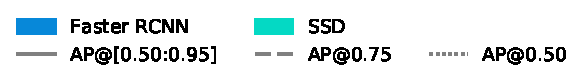
\includegraphics[scale=1]{graphics/matplot/img-detection__legend_3.pdf}
  \begin{subfigure}[t]{0.5\linewidth}
    \centering
    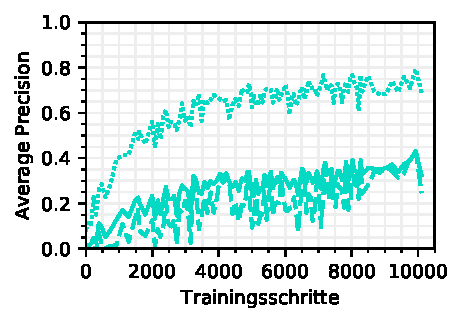
\includegraphics[scale=1]{graphics/matplot/img-detection__all__ap__train.pdf}
    \subcaption{Average Precision auf den Trainingsdaten} 
    \label{fig:3ap-map:map_train}
    \vspace{2ex}
  \end{subfigure}%% 
  \begin{subfigure}[t]{0.5\linewidth}
    \centering
    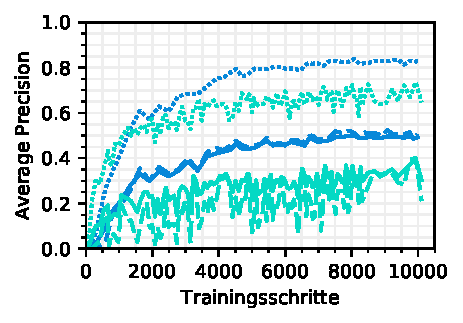
\includegraphics[scale=1]{graphics/matplot/img-detection__all__ap.pdf}
    \subcaption{Average Precision auf den Validierungsdaten} 
    \label{fig:3ap-map:map_val}
    \vspace{2ex}
  \end{subfigure}
\end{figure}

\todo[inline]{train SSD on smaller LR to reduce the jumping in the graph...}

Abbildung \ref{fig:3ap-map:loss} zeigt das Loss der beiden Modelle auf den Validierungsdaten über den Trainingsverlauf hinweg. Es ist zu erkennen, dass das Loss nach 4000 Trainingsschritten schon sehr flach wird. Die Modelle Lernen zu diesem Zeitpunkt also nur noch sehr wenig. Die Modelle noch weiter zu trainieren, würde keine Verbesserung der Mean Average Precision zur Folge haben.

\todo[inline]{Use single figsize for the following graphic}

\begin{figure}[h!] 
%\begin{wrapfigure}{r}{0.5\textwidth} 
    \captionsetup{width=.9\linewidth}
    \caption{TODO: Totales loss auf den Validierungsdaten}
    \label{fig:3ap-map:loss}
    \centering
    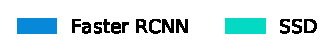
\includegraphics[scale=1]{graphics/matplot/img-detection__legend_1.pdf}
    
    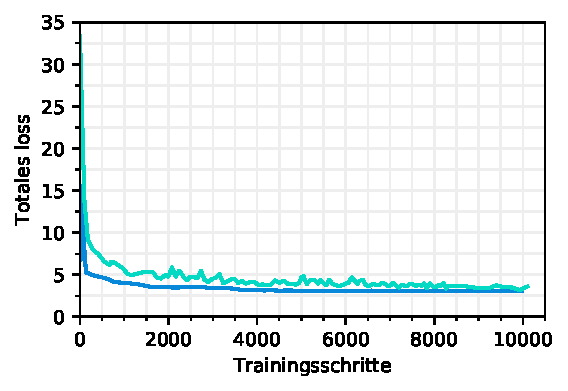
\includegraphics[scale=1]{graphics/matplot/img-detection__all__loss.pdf}
%\end{wrapfigure}
\end{figure}

Einen etwas detaillierteren Einblick in die Qualität der Modelle gibt die Tabelle \ref{tab:3ap-iou}. Die Tabelle zeigt die Durchschnittliche Intersection over Union Metrik der beiden Modelle für die einzelnen zu erkennenden Klassen. Dabei ist festzustellen, dass die beiden Modelle die Adresse des Patienten sowie die Rechnungspositionen relativ gut erkennen können. Bei den anderen beiden Klassen sind die Resultate dagegen ernüchternd.

Auffällig an der Gegenüberstellung der Mean IoU Werte ist die Klasse Totalbetrag. Dabei schneidet das SSD Modell extrem schlecht ab. Das SSD Modell scheint mit dieser Flächen mässig kleinen Region of Interest also besonders Probleme zu haben.

\begin{table}[h!]
\label{tab:3ap-iou}
\centering
    \captionsetup{width=.9\linewidth}
    \caption{Durchschnittliche Intersection over Union der einzelnen Klassen}
    \begin{tabular}{lll}
                                    & \multicolumn{2}{c}{\textbf{Modell}}  \\
    \textbf{Klasse}                          & \textbf{Faster-RCNN} & \textbf{SSD}           \\
    Adresse des Patienten           & 0.850       & 0.731         \\
    Adresse des Leistungserbringers & 0.625       & 0.623         \\
    Rechnungspositionen             & 0.835       & 0.728         \\
    Totalbetrag                     & 0.629       & 0.258             
    \end{tabular}
\end{table}

Subsummierend kann festgehalten werden, dass das Faster-RCNN Modell erwartungsgemäss präzisere Vorhersagen macht. 

In Bezug auf die Automatisierung der Rechnungseinreichung sind die Adresse des Patienten sowie das Total der Rechnung relevant. Das präsentierte Modell kann aber nur eine der beiden Informationen mit einer hohen Genauigkeit erkennen. Weiter fehlen noch andere relevante Informationen wie das Datum des Bezugs der Leistung sowie die Aussage, ob eine Ärztliche Verordnung vorliegt oder nicht. 

Im folgenden Kapitel wird versucht diesen Ansatz um die fehlenden Informationen zu ergänzen sowie die Qualität der Ergebnisse zu steigern, indem das Modell auf Rechnungen bestimmter Leistungserbringer spezialisiert wird.

\todo[inline, color=igloo]{
- Rechnungen mit erkannten Regions als Beispiele zeigen, sieht cool aus
}

\subsubsection{Bild-basierte Informationsextraktion pro Rechnungstyp}
In diesem Kapitel wird der bild-basierte Ansatz zur Informationsextraktion, welcher im vorherigen Kapitel beschrieben wurde, auf Rechnungen eines einzelnen Leistungserbringers (beispielsweise Fielmann) angewendet. Dadurch wird erhofft ein besseres Resultat erzielen zu können. Des weiteren werden die zu erkennenden Region of Interest so angepasst, dass sich diese mit den Anforderungen aus dem Kapitel \ref{chap:requirements} decken. Das bedeutet, dass neu die Positionen der Klassen Adresse des Patienten, Adresse des Leistungserbringers, Datum des Leistungsbezuges, Totalbetrag und Begründung des Leistungsbezuges (mögliche ärztliche Verschreibung) erkannt werden sollen.

Damit in der Praxis spezifische Modelle zur Informationsextraktion auf die Rechnungen der einzelnen Leistungserbringer angewendet werden können, muss das Modell zur Klassifizierung der Rechnung um die Klassen dieser Leistungserbringer erweitert werden. Nachfolgend wird diese Erweiterung des Modells zur Klassifizierung sowie die Erstellung des Leistungserbringer-spezifischen bild-basierten Modell zur Informationsextraktion beschrieben und die Resultate daraus diskutiert.

Das im Kapitel \ref{chap:text-based-classification} beschriebene, text-basierte Modell zur Klassifizierung der Rechnungen wurde um die Klassen Fielmann und Visilab erweitert. Diese Klassen wurden gewählt, da sie innerhalb der aktuell grössten Klasse von Rechnungen, der Klasse Optiker, einen grossen Anteil haben. Es stehen 578 Rechnungen von Fielmann sowie 195 Rechnungen von Visilab zur Verfügung.

Die Abbildung \ref{fielmann-cm} zeigt die Confusion Matrix des angepassten Modells auf den Validierungsdaten. Darauf ist zu erkennen, dass die Einteilung in die beiden neuen Klassen sehr gut funktioniert. Nach 45 Epochen Training werden innerhalb des Validierungsdatensatzes lediglich 2 Rechnungen fälschlicherweise als Visilab Rechnungen klassifiziert. Diese Klassifizierung ist nicht per se falsch, denn es handelt sich tatsächlich um Rechnungen von Visilab, aber in einem anderen Format: ein Kassenbeleg sowie eine Monatsrechnung. Diese Unterschiede im Format würden nicht in das erwartete Muster des im zweiten Schritt folgenden Modell zur Informationsextraktion passen und werden deshalb in diesem Fall als Falsch angesehen.

\begin{figure}[h!] 
%\begin{wrapfigure}{r}{0.5\textwidth} 
    \captionsetup{width=.9\linewidth}
    \caption[Confusion Matrix des um die Klassen Fielmann und Visilab ergänzten text-basierten Modells zur Klassifizierung von Rechnungen]{Confusion Matrix nach 45 Epochen Training des erweiterten text-basierten Modells zur Klassifizierung von Rechnungen.}
    \label{fielmann-cm}
    \centering
    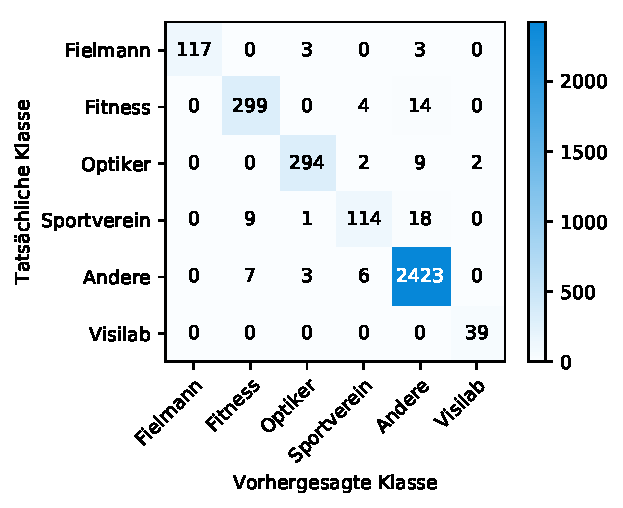
\includegraphics[scale=1]{graphics/matplot/class__fielmann__cm_44.pdf}
%\end{wrapfigure}
\end{figure}

Das Faster-RCNN und SSD Modell wurden auf den Rechnungen der Klassen Fielmann und Visilab trainiert. Die Abbildung \ref{fig:specific-ie} zeigt die Mean Average Precisions der beiden Modelle für verschiedene IoU Schwellwerte für die beiden Klassen.

\begin{figure}[h!] 
  \captionsetup{width=.9\linewidth}
  \caption{TODO}
  \label{fig:specific-ie}
  \centering
  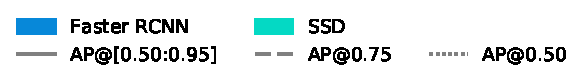
\includegraphics[scale=1]{graphics/matplot/img-detection__legend_3.pdf}
  \begin{subfigure}[b]{0.45\linewidth}
    \centering
    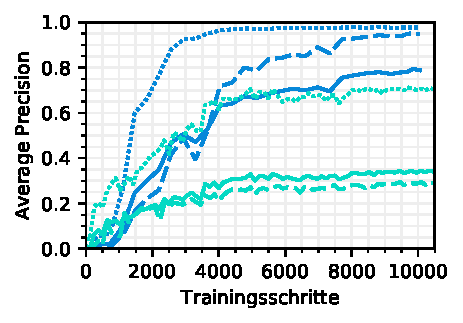
\includegraphics[scale=1]{graphics/matplot/img-detection__fielmann__ap__train.pdf}
    \caption{Average Precision auf den Trainingsdaten der Klasse Fielmann} 
    \label{fig:specific-ie:fielmann:ap_train}
    \vspace{2ex}
  \end{subfigure}%% 
  \begin{subfigure}[b]{0.45\linewidth}
    \centering
    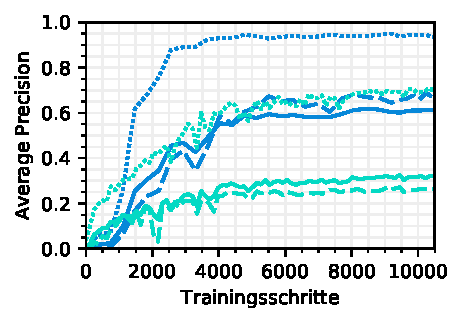
\includegraphics[scale=1]{graphics/matplot/img-detection__fielmann__ap.pdf}
    \caption{Average Precision auf den Validierungsdaten der Klasse Fielmann} 
    \label{fig:specific-ie:fielmann:ap_val}
    \vspace{2ex}
  \end{subfigure}
  \begin{subfigure}[b]{0.45\linewidth}
    \centering
    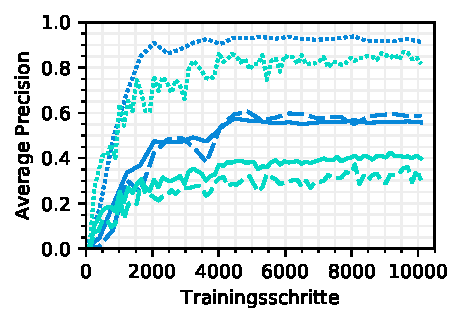
\includegraphics[scale=1]{graphics/matplot/img-detection__visilab__ap.pdf}
    \caption{Average Precision auf den Trainingsdaten der Klasse Visilab} 
    \label{fig:specific-ie:visilab:ap_train}
    \vspace{2ex}
  \end{subfigure}%%
  \begin{subfigure}[b]{0.45\linewidth}
    \centering
    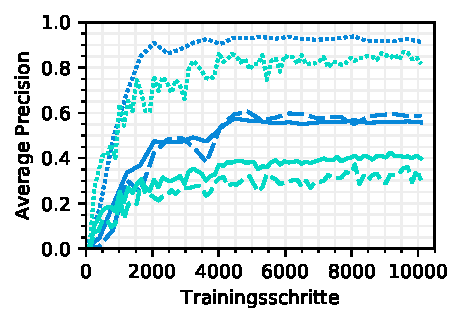
\includegraphics[scale=1]{graphics/matplot/img-detection__visilab__ap.pdf}
    \caption{Average Precision auf den Validierungsdaten der Klasse Visilab} 
    \label{fig:specific-ie:visilab:ap_val}
    \vspace{2ex}
  \end{subfigure}
\end{figure}

Die Abbildung \ref{fig:specific-ie:loss} zeigt das Loss der beiden Modelle auf den Validierungsdaten für beide Klassen. Es ist zu erkennen, dass die Modelle auch auf den Leistungserbringer spezifischen Rechnungen nach ca. 4000 Trainingsschritten nicht mehr stark lernen. Die Modelle weiter zu trainieren, dürfte auch hier keine Erhöhung der Mean Average Precisions mehr zur Folge haben.

\begin{figure}[h!] 
  \captionsetup{width=.9\linewidth}
  \label{fig:specific-ie:loss}
  \caption{TODO}
  \centering
  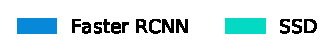
\includegraphics[scale=1]{graphics/matplot/img-detection__legend_1.pdf}
  \begin{subfigure}[b]{0.45\linewidth}
    \centering
    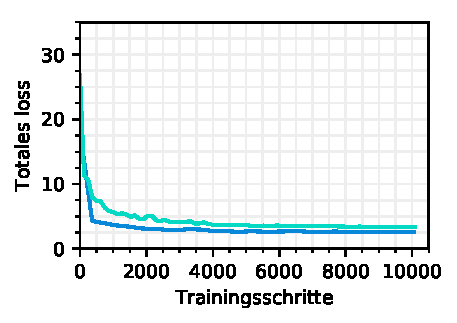
\includegraphics[scale=1]{graphics/matplot/img-detection__fielmann__loss.pdf}
    \caption{Totales loss auf den Validierungsdaten der Klasse Fielmann} 
    \label{fig:specific-ie:visilab:loss}
    \vspace{2ex}
  \end{subfigure}%% 
  \begin{subfigure}[b]{0.45\linewidth}
    \centering
    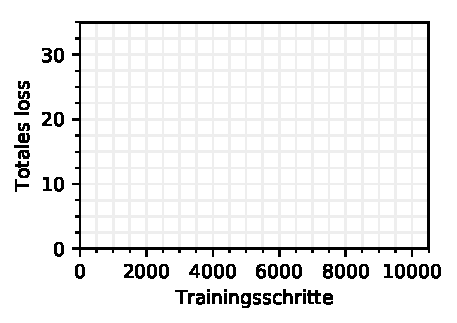
\includegraphics[scale=1]{graphics/matplot/img-detection__visilab__loss.pdf}
    \caption{Totales loss auf den Validierungsdaten der Klasse Visilab} 
    \label{fig:specific-ie:visilab:loss}
    \vspace{2ex}
  \end{subfigure} 
\end{figure}

\todo[inline, color=igloo]{Use package hhline to fix border issues...}

\begin{table}[h!]
\label{tab:specific-ie-iou}
\centering
    \captionsetup{width=.9\linewidth}
    \caption{Durchschnittliche Intersection over Union der einzelnen Klassen}
    %\begin{tabular}{lllll}
    \begin{tabular}{|l|l|l|l|l|}
    \hline
                                    & \multicolumn{4}{c}{\textbf{Modell}}  \\
    \hline
                                    & \multicolumn{2}{c}{\textbf{Fielmann}} & \multicolumn{2}{c}{\textbf{Visilab}} \\
    \hline
    \textbf{Region of Interest}     & \textbf{Faster-RCNN}   & \textbf{SSD}        & \textbf{Faster-RCNN}  & \textbf{SSD} \\
    %                                & \textbf{(Fielmann)}   & \textbf{(Fielmann)}        & \textbf{(Visilab)}  & \textbf{(Visilab)} \\
    \hline
    Adresse des            &                        & 0.884                & & \\
    Patienten &&&& \\
    \hline
    Adresse des  &                        & 0.692                & & \\
    Leistungserbringers &&&& \\
    \hline
    Begründung des  &                        & 0.716                & & \\
    Leistungsbezuges &&&& \\
    \hline
    Totalbetrag                     &                        & 0.672                & & \\
    \hline
    \end{tabular}
\end{table}


\subsubsection{Weitere Ansätze}

\todo[inline]{
- CBR-DIA aus https://ieeexplore.ieee.org/stamp/stamp.jsp?arnumber=4378726

% Siehe reddit comment unter Eigener Ansatz

- Im selben reddit thread wie oben erwähnt werden weitere Lösungsansätze dargestellt

-- Simple solution: Classify each word into binary: total/not total. Dream up some features, e.g. various regex rules, adjecent words, etc. Pick word w. Highest prob.

--- just using adjacent words with CountVectorizer as the features, this seems to work really well

-- Fancy solution: treat it as a neural translation task from your input sequence of words to a single word output (the total) and use RNNs.


- https://www.diva-portal.org/smash/get/diva2:934351/FULLTEXT01.pdf

-- Naive Bayes for feature classification

-- Support Vector Machines -> Geht in Richtung Eigener Ansatz


- Online Lösungen

-- https://www.taggun.io, https://rossum.io

-- Rossum hat ein Team, welches sich nur um Data Annotation kümmert: https://rossum.ai/blog/rossums-training-data/

- Lösungen von FiBu Software
}
%TC:endignore